\subsection{Integrated Rank Weighted Depth}
\label{section:IRWD}

\begin{figure}[t]
    \centering
    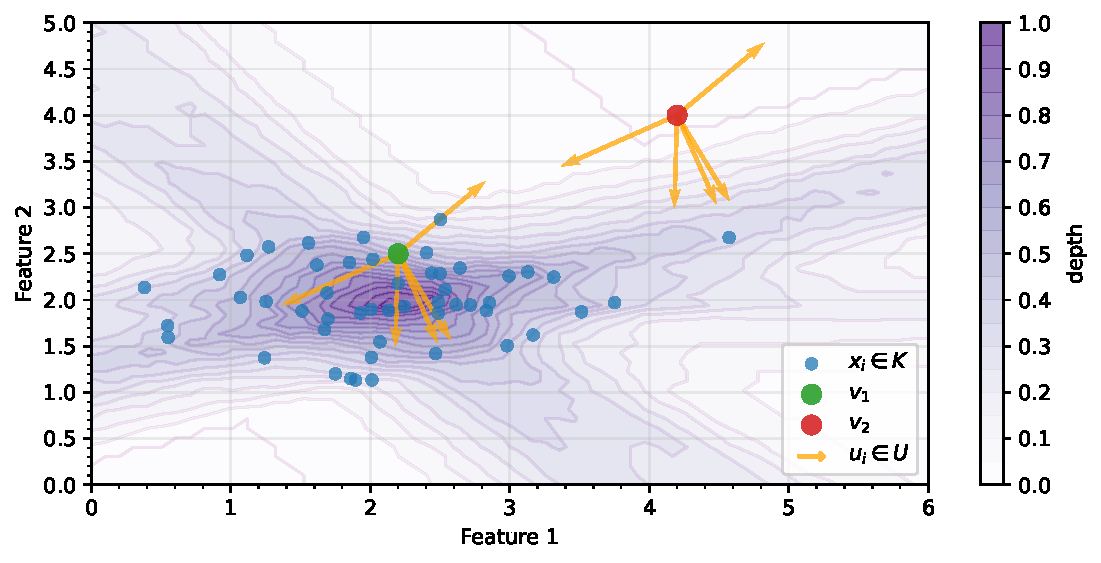
\includegraphics[width=\textwidth]{images/measures/irwd-distance.pdf}
    \caption{Idea of the Integrated Rank Weighted Depth applied as an outlierness measure.
             The contour plot is used to visualize the depths calculated for cluster $T$.
             Point $v_1$ is located in the region surrounded by cluster $T$ points (high depth),
             while point $v_2$ is an outlier (low depth value). The projection vectors $u_i$ involved in depth calculation are drawn for reference. The depth values are normalized for convenience.}
    \label{fig:irwd-idea}
\end{figure}

\begin{figure}[t]
    \centering
    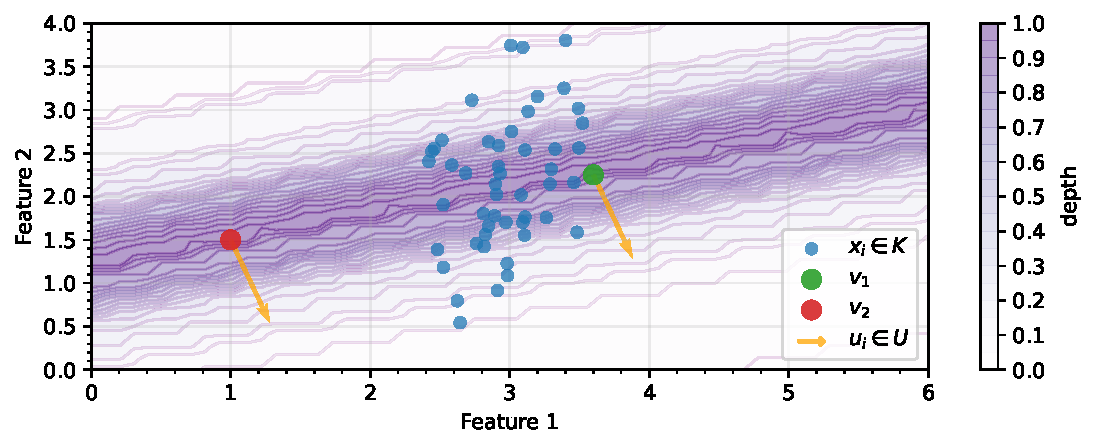
\includegraphics[width=\textwidth]{images/measures/irwd-issue.pdf}
    \caption{The IRWD algorithm identifying spurious correlation due to $n_{proj} < d$.\\
             In this case, element $v_2$ is considered as close to the cluster $T$ as the element $v_1$.
             Utilizing more projection vectors $u_i$ would help mitigating the problem.}
    \label{fig:irwd-issue}
\end{figure}

The Integrated Rank Weighted Depth, published by Ramsay et al. \cite{Ramsay-2019}, is another method of quantifying the outlierness score. It utilizes the Monte Carlo-like approach and considers angles between feature vectors for producing a representation of the known/training set, with the similarity then determined using so called depth of data.

First, a collection $U$ of $n_{proj}$ number of projection vectors $u_j$ is created by randomly selecting directions from a unit hyper-sphere in $\mathbb{R}^d$ space. Then, a representation of known data cluster $T$ is prepared by computing matrix $M$ of size $n_{T} \times n_{proj}$, containing the scalar products between each feature vector $x_i \in T$ and projection vector $\vv{u_j} \in U$,
\begin{equation}
    M[i, j] = x_i \cdot u_j
    ~.
    \label{eq:irwd-M}
\end{equation}

Each $i$-th row in matrix $M$ corresponds to the feature vector $x_i$ of cluster $T$, while each $j$-th column corresponds to the scalar products values obtained for the projection vector $u_j$. Hence, there are $n_{T}$ rows and $n_{proj}$ columns; the $M[i, j]$ component is a~value of the scalar product between vectors $x_i$ and $u_j$.

To calculate the outlierness score for a given vector $v$ against the data cluster $T$, the next step to compute the values of scalar products between $v$ and the projection vectors $u_j \in U$, then subtracting the resulting values from the representation matrix $M$,
\begin{equation}
    M_v[i, j] = M[i, j] - v \cdot u_j
    ~.
    \label{eq:irwd-M_v}
\end{equation}

The resulting matrix $M_v$ is processed column-wise, which corresponds to analyzing results obtained for each projection vector $u_j$. For each column, the number of positive and negative values is counted and the lower number is selected. Finally, the outlierness score is calculated as a sum of selected numbers, divided by the number of $M_v$ elements,
\begin{equation}
    IRWD(v, T)
    =
    \frac{1}{n_{T}}
    \cdot
    \frac{1}{n_{proj}}
    \cdot
    \sum_{j=1}^{n_{proj}}
    \min\big\{
        ~
        \mathrm{count}\{M[*,j] \le 0\}
        ~,~
        \mathrm{count}\{M[*,j] > 0\}
        ~
    \big\}
    ~.
    \label{eq:irwd}
\end{equation}

Intuitively, the values of $M_v$ matrix correspond to the distances and locations of each feature vector $x_i$ in relation to the given $v$ while looking along the direction $u_j$. In~other words, when considering a plane defined by a point $v$ and a vector $u_j$, the positive value of $M_v[i,j]$ means that given $x_i$ is in front/above that plane, while the negative value means the $x_i$ is behind such plane. Note that the actual individual distance itself is not relevant, there matters only the location that is linked to the sign (positive/negative) of the distance value. The score gets maximized, if there is an equal number of elements $x_i$ on both sides of the plane. Hence, the idea of the data depth emerges as a way of characterizing and localizing the center of a~distribution, which is promised to be suitable especially for non-Gaussian distributions, where only the traditional mean and median may not provide reliable understanding of data spread.

The high depth value indicates that a data point $v$ lies within the central region of the data cluster $T$, surrounded by neighbors. Contrary, low depth value suggests that a~point is located on the outskirts of the data distribution, potentially indicating that the $v$ may by an outlier. Figure \ref{fig:irwd-idea} illustrates both such cases with the random projection vectors $u_i$ drawn for the reference as well.

It is worth to notice that the chosen number of random projection vectors, $n_{proj}$, impacts the outcome of IRWD significantly. Especially, with $n_{proj}$ lower than the dimension of $\mathbb{R}^d$ space, i.e., $n_{proj} < d$, there is a risk of identifying spurious correlations in data. Example of the such case was presented in the figure \ref{fig:irwd-issue}, where both in-distribution data ($v_1$) and the out-of-distribution sample ($v_2$) are ranked with the same depth score.

During the research the own implementation (Section \ref{section:pyopenset}) was used, based on the description from the the NeurIPS publication \cite{Colombo-2022}. For convenience, the returned values were inverted, so the greater values indicate that data more likely to be outliers.
